\section{Introduktion}

\subsection{Ern\"{o} Rubik}
\begin{frame}{Ern\"{o} Rubik}
\begin{itemize}
	\item<1>Ungarn
	\item<1>1944
	\item<1>Ingeni�r 
\end{itemize}
\end{frame}

\subsection{Rubik's Terningen}
\begin{frame}{Rubik's Terningen}
\begin{itemize}
	\item<1>27 cubies
	\item<1>6 faces
	\item<1>9 facelets
\end{itemize}
\begin{figure}[bp]
	\centering
		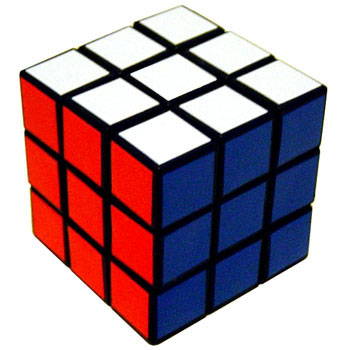
\includegraphics[scale=0.25]{input/pics/rubiks-cube.jpg}
	%\caption{En l�st Rubik's terning}
	\label{fig:rubiks-cube}
\end{figure}

\end{frame}